\frame{\frametitle{European Space Agency}
\vspace{-0.1cm}
\centering
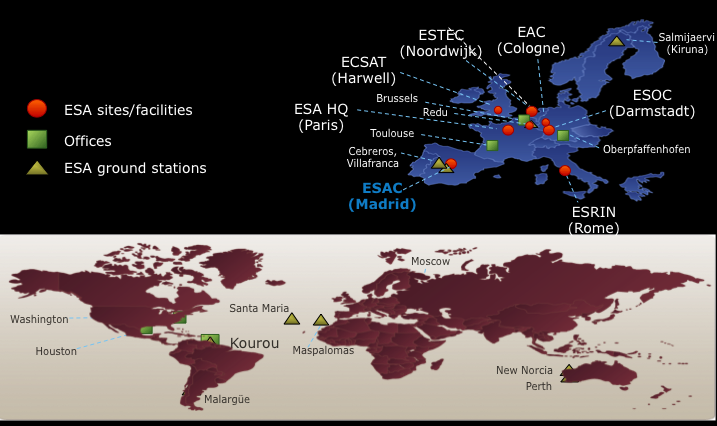
\includegraphics[width=0.9\textwidth]{esaloc}
}

\frame{\frametitle{European Spacecraft Operations Centre}
\vspace{3pt}
\begin{columns}[c]
\column{0.5\textwidth}
Late 1990s SCOSII software contractors
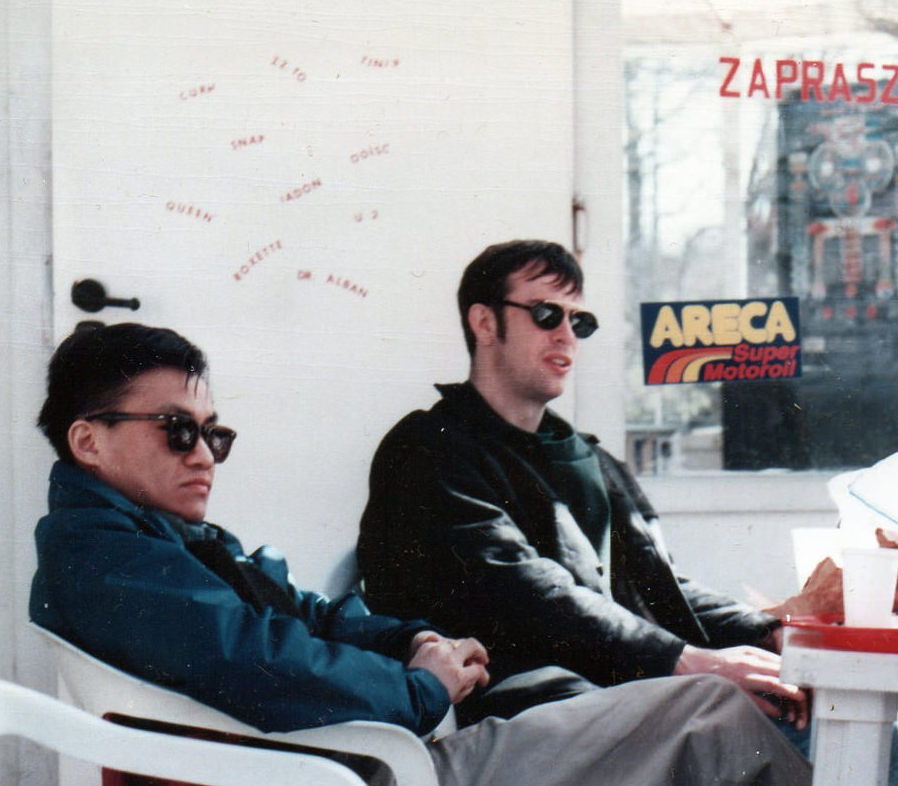
\includegraphics[width=\textwidth]{wom96}
\column{0.5\textwidth}
\begin{itemize}
\item ESOC - Located in Darmstadt, near Frankfurt, Germany.
\item Controls all ESA satellites.
\item System design/engineering, requirements management, advanced studies ..
\item  SCOSII (Satellite Control and Operations System) for ENVISAT

\end{itemize}
\end{columns}
}

\frame{\frametitle{European Space Technology Research  Centre}
\begin{columns}[c]
\column{0.5\textwidth}
 1998 Integral in ESTEC
\vspace{-1cm}
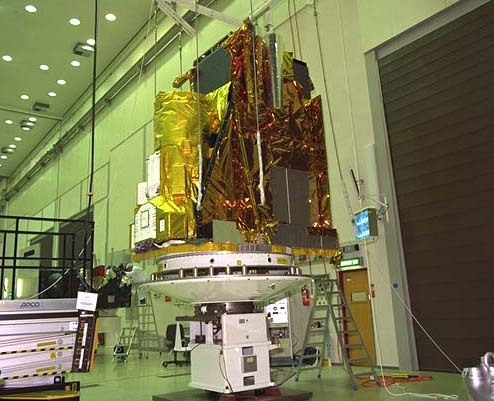
\includegraphics[width=\textwidth]{int98}\\
\column{0.5\textwidth}
\begin{itemize}
\item ESTEC - Located near Noordwijk, Netherlands.
\item Worked on Hipparcos, Integral, Planck and Gaia study phase:
\begin{itemize}
\item First ideas on Global Astrometric Solution \citep{1999BaltA...8...57O} and {\color{red} how to make a consortium}.
\item How to tessellate the celestial  sphere : HEALPix and HTM work proved popular \citep{2001misk.conf..638O}.
\end{itemize}
\end{itemize}
\end{columns}
}

\frame{\frametitle{Addition to HIP Catalogue}
1997/98 Hipparcos Java Tools - learning Astrometry
\url{http://www.cosmos.esa.int/web/hipparcos/java-tools}
\includegraphics[width=\textwidth]{hipjt}
}


\frame{\frametitle{In the USA early 2000s}
\vspace{5pt}
\begin{columns}[c]
\column{0.6\textwidth}
Entering the new millennium ..  \\
\vspace{4pt}
Quality tools for GSC2 (Java) $\rightarrow$\\
\vspace{8pt}
CasJobs (C\#)\citep{2004ASPC..314..372O}
\includegraphics[width=\textwidth]{casjobs}
\column{0.4\textwidth}
\includegraphics[width=\textwidth]{sshtm}
\vspace{-1cm}
\includegraphics[width=\textwidth]{showsky}
\end{columns}
}


\frame{\frametitle{European Space Astronomy Centre}
\begin{columns}[c]
\column{0.4\textwidth}
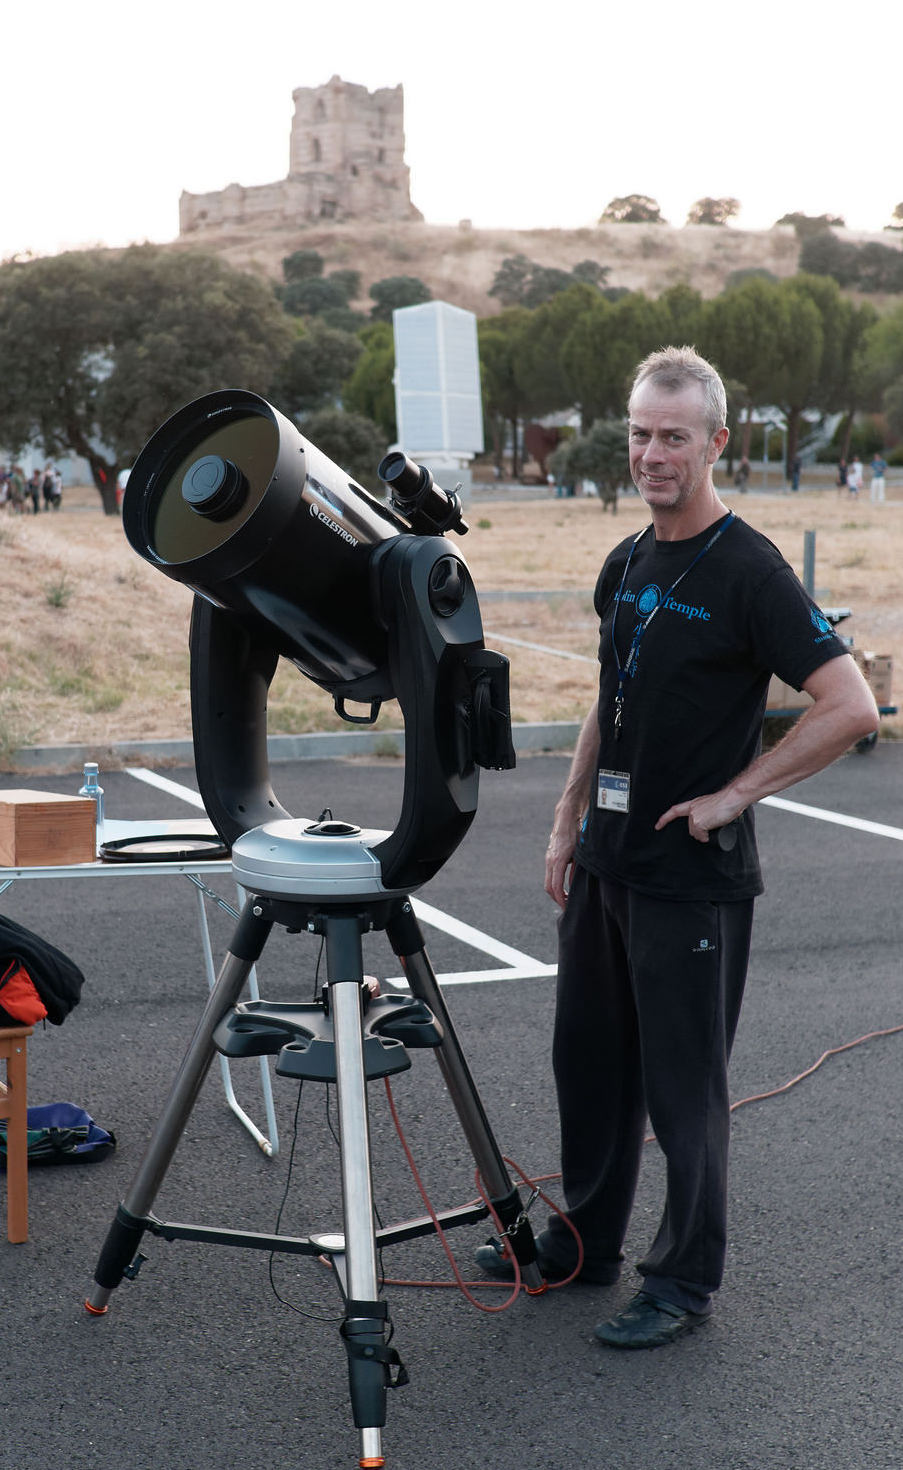
\includegraphics[width=\textwidth]{wom2016}\\
\column{0.6\textwidth}
\vspace{-1cm}
 \\
From 2005 to 2017\\
\begin{itemize}
\item ESAC Located near Madrid, Spain.
\item Home of the Science Operations Department of the European Space Agency
\item Surprising number of Irish people ..
\item This picture from a public stargazing night - $\sim$400 visitors came

\end{itemize}
\end{columns}
}


\frame{\frametitle{Visitors to ESAC 2013 }
\centering

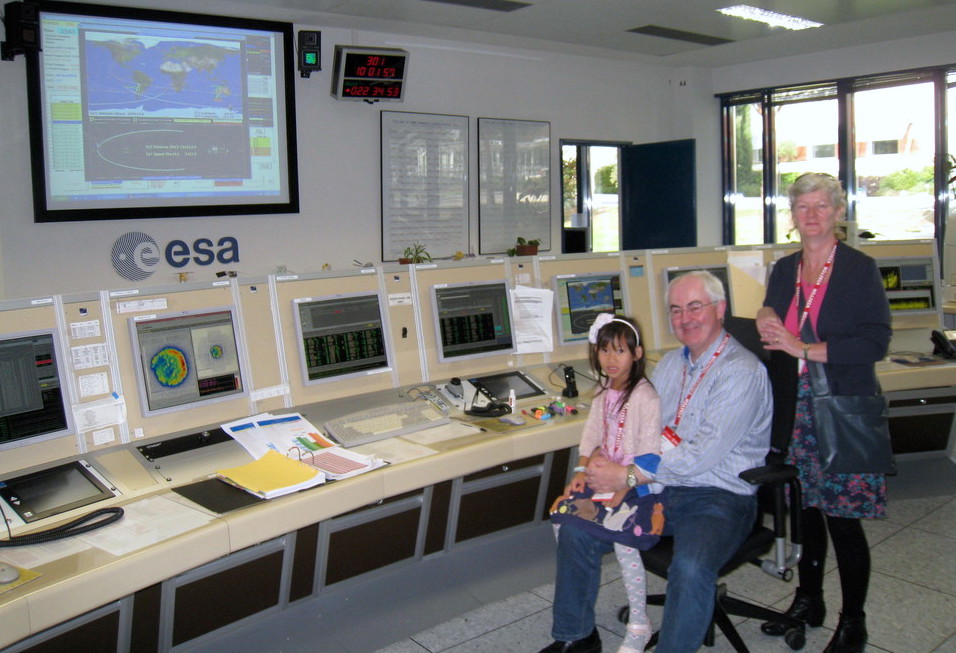
\includegraphics[width=0.75\textwidth]{figures/ainecEsac}
}

